% This is the Reed College LaTeX thesis template. Most of the work
% for the document class was done by Sam Noble (SN), as well as this
% template. Later comments etc. by Ben Salzberg (BTS). Additional
% restructuring and APA support by Jess Youngberg (JY).
% Your comments and suggestions are more than welcome; please email
% them to cus@reed.edu
%
% See http://web.reed.edu/cis/help/latex.html for help. There are a
% great bunch of help pages there, with notes on
% getting started, bibtex, etc. Go there and read it if you're not
% already familiar with LaTeX.
%
% Any line that starts with a percent symbol is a comment.
% They won't show up in the document, and are useful for notes
% to yourself and explaining commands.
% Commenting also removes a line from the document;
% very handy for troubleshooting problems. -BTS

% As far as I know, this follows the requirements laid out in
% the 2002-2003 Senior Handbook. Ask a librarian to check the
% document before binding. -SN

%%
%% Preamble
%%
% \documentclass{<something>} must begin each LaTeX document

\documentclass[oneside]{report}
\usepackage{Suthesis-2e}
% Packages are extensions to the basic LaTeX functions. Whatever you
% want to typeset, there is probably a package out there for it.
% Chemistry (chemtex), screenplays, you name it.
% Check out CTAN to see: http://www.ctan.org/
%%
\usepackage{graphicx,latexsym}
\usepackage{amsmath}
\usepackage{amssymb,amsthm}
\usepackage{longtable,booktabs,setspace}
\usepackage{chemarr} %% Useful for one reaction arrow, useless if you're not a chem major
\usepackage[hyphens]{url}
% Added by CII
\usepackage[draft]{hyperref}
\usepackage{lmodern}
\usepackage{float}
\floatplacement{figure}{H}
% End of CII addition
\usepackage{rotating}

% Next line commented out by CII
%%% \usepackage{natbib}
% Comment out the natbib line above and uncomment the following two lines to use the new
% biblatex-chicago style, for Chicago A. Also make some changes at the end where the
% bibliography is included.
%\usepackage{biblatex-chicago}
%\bibliography{thesis}


% Added by CII (Thanks, Hadley!)
% Use ref for internal links
\renewcommand{\hyperref}[2][???]{\autoref{#1}}
\def\chapterautorefname{Chapter}
\def\sectionautorefname{Section}
\def\subsectionautorefname{Subsection}
% End of CII addition

% Added by CII
\usepackage{caption}
\captionsetup{width=5in}
% End of CII addition

% \usepackage{times} % other fonts are available like times, bookman, charter, palatino

% Syntax highlighting #22

% Added by KM to include latex packages
	\usepackage{array}
	\usepackage{float}
	\usepackage{tabularx}
	\usepackage{longtable}

% To pass between YAML and LaTeX the dollar signs are added by 
\setstretch{1.6}
\begin{document}
\title{Children's flexible information seeking during language comprehension
and word learning}
\author{Kyle MacDonald}
% The month and year that you submit your FINAL draft TO THE LIBRARY (May or December)
\date{November 2018}
\dept{Psychology}
\principaladviser{Michael C. Frank}
\firstreader{Hyowon Gweon}
\secondreader{James McClelland}
  \thirdreader{Virginia A. Marchman} %if needed

% if you're writing a thesis in an interdisciplinary major,
% uncomment the line below and change the text as appropriate.
% check the Senior Handbook if unsure.
%\thedivisionof{The Established Interdisciplinary Committee for}
% if you want the approval page to say "Approved for the Committee",
% uncomment the next line
%\approvedforthe{Committee}

% Added by CII
%%% Copied from knitr
%% maxwidth is the original width if it's less than linewidth
%% otherwise use linewidth (to make sure the graphics do not exceed the margin)
\makeatletter
\def\maxwidth{ %
  \ifdim\Gin@nat@width>\linewidth
    \linewidth
  \else
    \Gin@nat@width
  \fi
}
\makeatother

\renewcommand{\contentsname}{Contents}
% End of CII addition

\setlength{\parskip}{0pt}

% Added by CII

\providecommand{\tightlist}{%
  \setlength{\itemsep}{0pt}\setlength{\parskip}{0pt}}




\beforepreface
\prefacesection{Abstract}
The preface pretty much says it all.

\par

Second paragraph of abstract starts here.

\prefacesection{Dedication}
You can have a dedication here if you wish.
%\prefacesection{}
%This thesis is dedicated to 
\prefacesection{Acknowledgments}
I want to thank a few people.

\afterpreface


\hypertarget{introduction}{%
\chapter*{Introduction}\label{introduction}}
\addcontentsline{toc}{chapter}{Introduction}

Language learning is remarkable.

\hypertarget{info-seeking}{%
\chapter{An information seeking account of eye
movements}\label{info-seeking}}

\hypertarget{sol}{%
\chapter{Real-time American Sign Language comprehension}\label{sol}}

\hypertarget{introduction-1}{%
\section[Introduction]{\texorpdfstring{Introduction\footnote{This
  chapter is published in MacDonald, LaMarr, Corina, Marchman, \&
  Fernald (2018). Real-time lexical comprehension in young children
  learning American Sign Language. \emph{Developmental science}, e12672.}}{Introduction}}\label{introduction-1}}

Finding meaning in a spoken or a signed language requires learning to
establish reference during real-time interaction -- relying on audition
to interpret spoken words, or on vision to interpret manual signs.
Starting in infancy, children learning spoken language make dramatic
gains in their efficiency in linking acoustic signals representing
lexical forms to objects in the visual world. Studies of spoken language
comprehension using the looking-while-listening (LWL) procedure have
tracked developmental gains in language processing efficiency by
measuring the timing and accuracy of young children's gaze shifts as
they look at familiar objects and listen to simple sentences (e.g.,
``Where's the ball?'') naming one of the objects (Fernald, Zangl,
Portillo, \& Marchman, 2008; Law \& Edwards, 2014; Venker, Eernisse,
Saffran, \& Ellis Weismer, 2013). Such research finds that eye movements
to named objects occur soon after the auditory information is sufficient
to enable referent identification, and often prior to the offset of the
spoken word (Allopenna, Magnuson, \& Tanenhaus, 1998). Moreover,
individual differences in the speed and accuracy of eye movements in
response to familiar words predict vocabulary growth and later language
and cognitive outcomes (Fernald, Perfors \& Marchman, 2006; Marchman \&
Fernald, 2008). Together, these results suggest that gaze shifts to
objects in response to spoken language reflect a rapid integration of
linguistic and visual information, and that variability in the timing of
these gaze shifts provides researchers a way to measure the efficiency
of the underlying integration process.

Much less is known about how language influences visual attention during
sign language comprehension, especially in young learners. Given the
many surface-level differences between signed and spoken languages, it
is not immediately clear whether the findings from spoken language will
generalize to signed languages or whether they are specific to
mechanisms of language comprehension in the auditory modality. In
particular, studies with children learning spoken languages find that
these skills undergo dramatic developmental changes over the 2nd and 3rd
years of life. Moreover, there are significant relations between
variation in efficiency in online language processing, as indexed by
language-driven eye movements, and measures of linguistic achievement,
such as vocabulary size and scores on standardized tests (Fernald et
al., 2006; Marchman \& Fernald, 2008). Will individual variation in
language processing among children learning a signed language also be
related to their age and vocabulary outcomes, as observed in children
learning a spoken language?

Here we address this question by developing precise measures of speed
and accuracy in real-time sign language comprehension by children
learning American Sign Language (ASL). First, we estimate the extent to
which adults and children tend to shift visual attention to a referent
and away from the language source prior to the offset of a sign naming
an object in the visual scene. Will signers wait until the end of the
signed utterance, perhaps to reduce the probability of missing upcoming
linguistic information? Or will signers shift gaze incrementally as the
signs unfold in time, initiating saccades soon after there is enough
information in the signal to identify the referent, similar to children
and adults processing spoken language? Another related possibility is
that signers would produce incremental gaze shifts to the named objects
while still monitoring the linguistic signal in the periphery. This
analysis provides an important first step towards validating the linking
hypothesis that eye movements generated in our task reflect efficiency
of sign recognition, rather than some other process, such as attending
to the objects after the process of sign comprehension is complete. If
children and adults produce rapid gaze shifts prior to target sign
offset, this would provide positive evidence of incremental ASL
processing.

Next, we compare the time course of ASL processing in deaf and hearing
native ASL-learners to ask whether having the potential to access
auditory information in their day-to-day lives would change the dynamics
of eye movements during ASL processing. Do deaf and hearing native
signers show parallel patterns of looking behavior driven by their
similar language background experiences and the in-the-moment
constraints of interpreting a sign language (i.e., fixating on a speaker
as a necessary requirement for gathering information about language)? Or
would the massive experience deaf children have in relying on vision to
monitor both the linguistic signal and the potential referents in the
visual world result in a qualitatively different pattern of performance
compared to hearing ASL learning, e.g., waiting until the end of the
sentence to disengage from the signer? This analysis is motivated by
prior work that has used comparisons between native hearing and deaf
signers to dissociate the effects of learning a visual-manual language
from the effects of lacking access to auditory information (e.g.,
Bavelier, Dye, \& Hauser, 2006).

Finally, we compare timing and accuracy of the eye movements of young
ASL-learners to those of adult signers, and ask whether there are
age-related increases in processing efficiency that parallel those found
in spoken languages. We also examine the links between variability in
children's ASL processing skills and their expressive vocabulary
development. A positive association between these two aspects of
language proficiency, as previously shown in children learning spoken
languages, provides important evidence that skill in lexical processing
efficiency is a language-general phenomenon that develops rapidly in
early childhood, regardless of language modality.

\hypertarget{asl-processing-in-adults}{%
\subsection{ASL processing in adults}\label{asl-processing-in-adults}}

Research with adults shows that language processing in signed and spoken
languages is similar in many ways. As in spoken language, sign
recognition is thought to unfold at both the lexical and sub-lexical
levels. Moreover, sign processing is influenced by both lexicality and
frequency; non-signs are identified more slowly than real signs (Corina
\& Emmorey, 1993) and high frequency signs are recognized faster than
low frequency signs (Carreiras, Gutiérrez-Sigut, Baquero, \& Corina,
2008). Recent work using eye-tracking methods found that adult signers
produce gaze shifts to phonological competitors, showing sensitivity to
sub-lexical features, and that these shifts were initiated prior to the
offset of the sign, showing evidence of incremental processing
(Lieberman, Borovsky, Hatrak, \& Mayberry, 2015). In addition, Caselli
and Cohen-Goldberg (2014) adapted a computational model, developed for
spoken language (Chen \& Mirman, 2012), to explain patterns of lexical
access in sign languages, suggesting that the languages share a common
processing architecture.

However, differences between spoken and signed languages in both
sub-lexical and surface features of lexical forms could affect the time
course of sign recognition (for reviews, see Carreiras, 2010 and Corina
\& Knapp, 2006). For example, Emmorey and Corina (1990) showed deaf
adults repeated video presentations of increasingly longer segments of
signs in isolation and asked them to identify the signs in an open-ended
response format. In the same study, English-speaking adults heard
repeated presentations of increasingly longer segments of spoken words.
Accurate identification of signs required seeing a smaller proportion of
the total sign length compared to words (see also Morford \& Carlsen,
2011), suggesting that features of visual-manual languages, such as
simultaneous presentation of phonological information, might increase
speed of sign recognition. Moreover, Gutierrez and colleagues (2012)
used EEG measures to provide evidence that semantic and phonological
information might be more tightly linked in the sign language lexicon
than in the spoken language lexicon. Thus there is evidence for both
similarities and dissimilarities in the processes underlying spoken-word
and manual-sign recognition. However, with a few exceptions
(e.g.~Lieberman et al., 2015, 2017), most of this work has relied on
offline methods that do not capture lexical processing as it unfolds in
time during naturalistic language comprehension. In addition, no
previous studies have characterized how young ASL-learners choose to
divide visual attention between a language source and the nonlinguistic
visual world during real-time language comprehension.

\hypertarget{lexical-development-in-asl}{%
\subsection{Lexical development in
ASL}\label{lexical-development-in-asl}}

Diary studies show that ASL acquisition follows a similar developmental
trajectory to that of spoken language (Lillo-Martin, 1999; Mayberry \&
Squires, 2006). For example, young signers typically produce
recognizable signs before the end of the first year and two-sign
sentences by their 2nd birthday (Newport \& Meier, 1985). And as in many
spoken languages (Waxman et al., 2013), young ASL-learners tend first to
learn more nouns than verbs or other predicates (Anderson \& Reilly,
2002). However, because children learning ASL must rely on vision to
process linguistic information and to look at named objects, it is
possible that basic learning processes, such as the coordination of
joint visual attention, might differ in how they support lexical
development (Harris \& Mohay, 1997). For example, in a study of book
reading in deaf and hearing dyads, Lieberman, Hatrak, and Mayberry
(2015) found that deaf children frequently shifted gaze to caregivers in
order to maintain contact with the signed signal. Hearing children, in
contrast, tended to look continuously at the book, rarely shifting gaze
while their caregiver was speaking. This finding suggests that the
modality of the linguistic signal may affect how young language learners
negotiate the demands of processing a visual language while
simultaneously trying to fixate on the referents of that language.

This competition for visual attention in ASL could lead to qualitatively
different looking behavior during real-time ASL comprehension, making
the link between eye movements and efficiency of language comprehension
in ASL less transparent. On the one hand, demands of relying on vision
to monitor both the linguistic signal and the named referent might cause
signers to delay gaze shifts to named objects in the world until the end
of the target sign, or even the entire utterance. In this case, eye
movements would be less likely to reflect the rapid, incremental
influence of language on visual attention that is characteristic of
spoken language processing. Another possibility is that ASL-learners,
like spoken language learners, will shift visual attention as soon as
they have enough linguistic information to do so, producing saccades
prior to the offset of the target sign. Evidence for incremental
language processing would further predict that eye movements during ASL
processing could index individual differences in speed of incremental
comprehension, as previously shown in spoken languages.

\hypertarget{research-questions}{%
\subsection{Research questions}\label{research-questions}}

Adapting the LWL procedure for ASL enables us to address four questions.
First, to what extent do children and adult signers shift their gaze
away from the language source and to a named referent prior to the
offset of the target sign? Second, how do deaf and hearing ASL-learners
compare in the time course of real-time lexical processing? Third, how
do patterns of eye movements during real-time language comprehension in
ASL-learners compare to those of adult signers? Finally, are individual
differences in ASL-learners' processing skill related to age and to
expressive vocabulary development?

\hypertarget{methods}{%
\section{Methods}\label{methods}}

Participants were 29 native, deaf and hearing ASL-learning children (17
females, 12 males) and 16 fluent adult signers (all deaf), as shown in
Table 1. Since the goal of the current study was to document
developmental changes in processing efficiency in native ASL-learners,
we set strict inclusion criteria. The sample consisted of both deaf
children of deaf adults and hearing Children of Deaf Adults (CODAs),
across a similar age range. It is important to note that all children,
regardless of hearing status, were exposed to ASL from birth through
extensive interaction with at least one caregiver fluent in ASL and were
reported to experience at least 80\% ASL in their daily lives.
Twenty-five of the 29 children lived in households with two deaf
caregivers, both fluent in ASL. Although the hearing children could
access linguistic information in the auditory signal, we selected only
ASL-dominant learners who used ASL as their primary mode of
communication both within and outside the home (10 out of 13 hearing
children had two deaf caregivers). Adult participants were all deaf,
fluent signers who reported using ASL as their primary method of
communication on a daily basis. Thirteen of the 16 adults acquired ASL
from their parents and three learned ASL while at school.

Our final sample size was determined by our success over a two-year
funding period in recruiting and testing children who met our strict
inclusion criteria -- receiving primarily ASL language input. It is
important to note that native ASL-learners are a small population. The
incidence of deafness at birth in the US is less than .003\%, and only
10\% of the 2-3 per 1000 children born with hearing loss have a deaf
parent who is likely to be fluent in ASL (Mitchell \& Karchmer, 2004).
In addition to the 29 child participants who met our inclusion criteria
and contributed adequate data, we also recruited and tested 17 more
ASL-learning children who were not included in the analyses, either
because it was later determined that they did not meet our stringent
criterion of exposure to ASL from birth (n = 12), or because they did
not complete the real-time language assessment due to inattentiveness or
parental interference (n = 5).

\begingroup\fontsize{12}{14}\selectfont
\begin{longtable}[t]{lrrrrr}
\caption[Age of ASL-learning children]{\label{tab:sol-demo-table}Age (in months) of hearing and deaf ASL-learning participants}\\
\toprule
\textbf{Hearing status} & \textbf{n} & \textbf{Mean} & \textbf{SD} & \textbf{Min} & \textbf{Max}\\
\midrule
deaf & 16 & 28.0 & 7.5 & 16 & 42\\
hearing & 13 & 29.4 & 11.2 & 18 & 53\\
\hline
all children & 29 & 28.6 & 9.2 & 16 & 53\\
\bottomrule
\end{longtable}\endgroup{}
\hypertarget{measures}{%
\subsection{Measures}\label{measures}}

Expressive vocabulary size: Parents completed a 90-item vocabulary
checklist, adapted from Anderson and Reilly (2002), and developed
specifically for this project to be appropriate for children between 1½
and 4 years of age. Vocabulary size was computed as the number of signs
reported to be produced by the child.

ASL Processing: Efficiency in online comprehension was assessed using a
version of the LWL procedure adapted for ASL learners, which we call the
Visual Language Processing (VLP) task. The VLP task yields two measures
of language processing efficiency, reaction time (RT) and accuracy.
Since this was the first study to develop measures of online ASL
processing efficiency in children of this age, several important
modifications to the procedure were made, as described below.

\hypertarget{procedure}{%
\subsection{Procedure}\label{procedure}}

The VLP task was presented on a MacBook Pro laptop connected to a 27''
monitor. The child sat on the caregiver's lap approximately 60 cm from
the screen, and the child's gaze was recorded using a digital camcorder
mounted behind the monitor. To minimize visual distractions, testing
occurred in a 5' x 5' booth with cloth sides. On each trial, pictures of
two familiar objects appeared on the screen, a target object
corresponding to the target noun, and a distracter object. All picture
pairs were matched for visual salience based on prior studies with
spoken language (Fernald et al., 2008). Between the two pictures was a
central video of an adult female signing the name of one of the
pictures. Participants saw 32 test trials with five filler trials (e.g.
``YOU LIKE PICTURES? MORE WANT?'') interspersed to maintain children's
interest.

Coding and Reliability. Participants' gaze patterns were video recorded
and later coded frame-by-frame at 33-ms resolution by highly-trained
coders blind to target side. On each trial, coders indicated whether the
eyes were fixated on the central signer, one of the images, shifting
between pictures, or away (off), yielding a high-resolution record of
eye movements aligned with target noun onset. Prior to coding, all
trials were pre-screened to exclude those few trials on which the
participant was inattentive or there was external interference. To
assess inter-coder reliability, 25\% of the videos were re-coded.
Agreement was scored at the level of individual frames of video and
averaged 98\% on these reliability assessments.

\hypertarget{stimuli}{%
\subsection{Stimuli}\label{stimuli}}

\emph{Linguistic stimuli.} To allow for generalization beyond
characteristics of a specific signer and sentence structure, we recorded
two separate sets of ASL stimuli. These were recorded with two native
ASL signers, using a different alternative grammatical ASL sentence
structures for asking questions (see Petronio and Lillo-Martin, 1997):
\begin{itemize}
\tightlist
\item
  Sentence-initial wh-phrase: ``HEY! WHERE {[}target noun{]}?''
\item
  Sentence-final wh-phrase: ``HEY! {[}target noun{]} WHERE?''
\end{itemize}
\noindent Each participant saw one stimulus set which consisted of one
ASL question structure, with roughly an even distribution of children
across the two stimulus sets (16 saw sentence-initial wh-phrase
structure; 13 saw the sentence-final wh-phrase structure).
\begin{table}

\caption[Iconicity scores and phonological overlap for ASL stimuli]{\label{tab:sol-asl-lex-table}Iconicity scores (1 = not iconic at all; 7 = very iconic) and degree of phonological overlap (out of 5 features) for each sign item-pair. Values were taken from ASL-LEX, a database of lexical and phonological properties of signs in ASL.}
\centering
\resizebox{\linewidth}{!}{
\begin{tabular}[t]{>{\raggedright\arraybackslash}p{3.5cm}>{\raggedleft\arraybackslash}p{3cm}l}
\toprule
\textbf{Item Pair (iconicity score 1-7)} & \textbf{Number of matched features} & \textbf{Matched features}\\
\midrule
bear (3.0) -- doll (1.2) & 1 & Movement\\
cat (4.6) -- bird (4.5) & 3 & Selected Fingers, Major Location, Sign Type\\
car (6.2) -- book (6.7) & 4 & Selected Fingers, Major Location, Movement, Sign Type\\
ball (5.7) -- shoe (1.5) & 4 & Selected Fingers, Major Location, Movement, Sign Type\\
\bottomrule
\end{tabular}}
\end{table}
To prepare the stimuli, two female native ASL users recorded several
tokens of each sentence in a child-directed register. Before each
sentence, the signer made a hand-wave gesture commonly used in ASL to
gain an interlocutor's attention before initiating an utterance. These
candidate stimuli were digitized, analyzed, and edited using Final Cut
Pro software, and two native signers selected the final tokens. The
target nouns consisted of eight object names familiar to most children
learning ASL at this age.

\emph{Visual stimuli.} The visual stimuli consisted of colorful
digitized pictures of objects corresponding to the target nouns
presented in four fixed pairs (cat---bird, car---book, bear---doll,
ball---shoe). See Table 2 for information about the degree of
phonological overlap in each item-pair and the degree of iconicity for
each sign (values were taken from ASL-LEX {[}Caselli et al.,
2017{]}).\footnote{We did not find evidence that these features were
  related to the speed or accuracy of participants' eye movements in our
  task. However, this study was not designed to vary these features
  systematically. See Appendix XX for the analysis.} Images were
digitized pictures presented in fixed pairs, matched for visual salience
with 3--4 tokens of each object type. Each object served as target four
times and as distracter four times for a total of 32 trials. Side of
target picture was counterbalanced across trials.
\begin{figure}[t]

{\centering 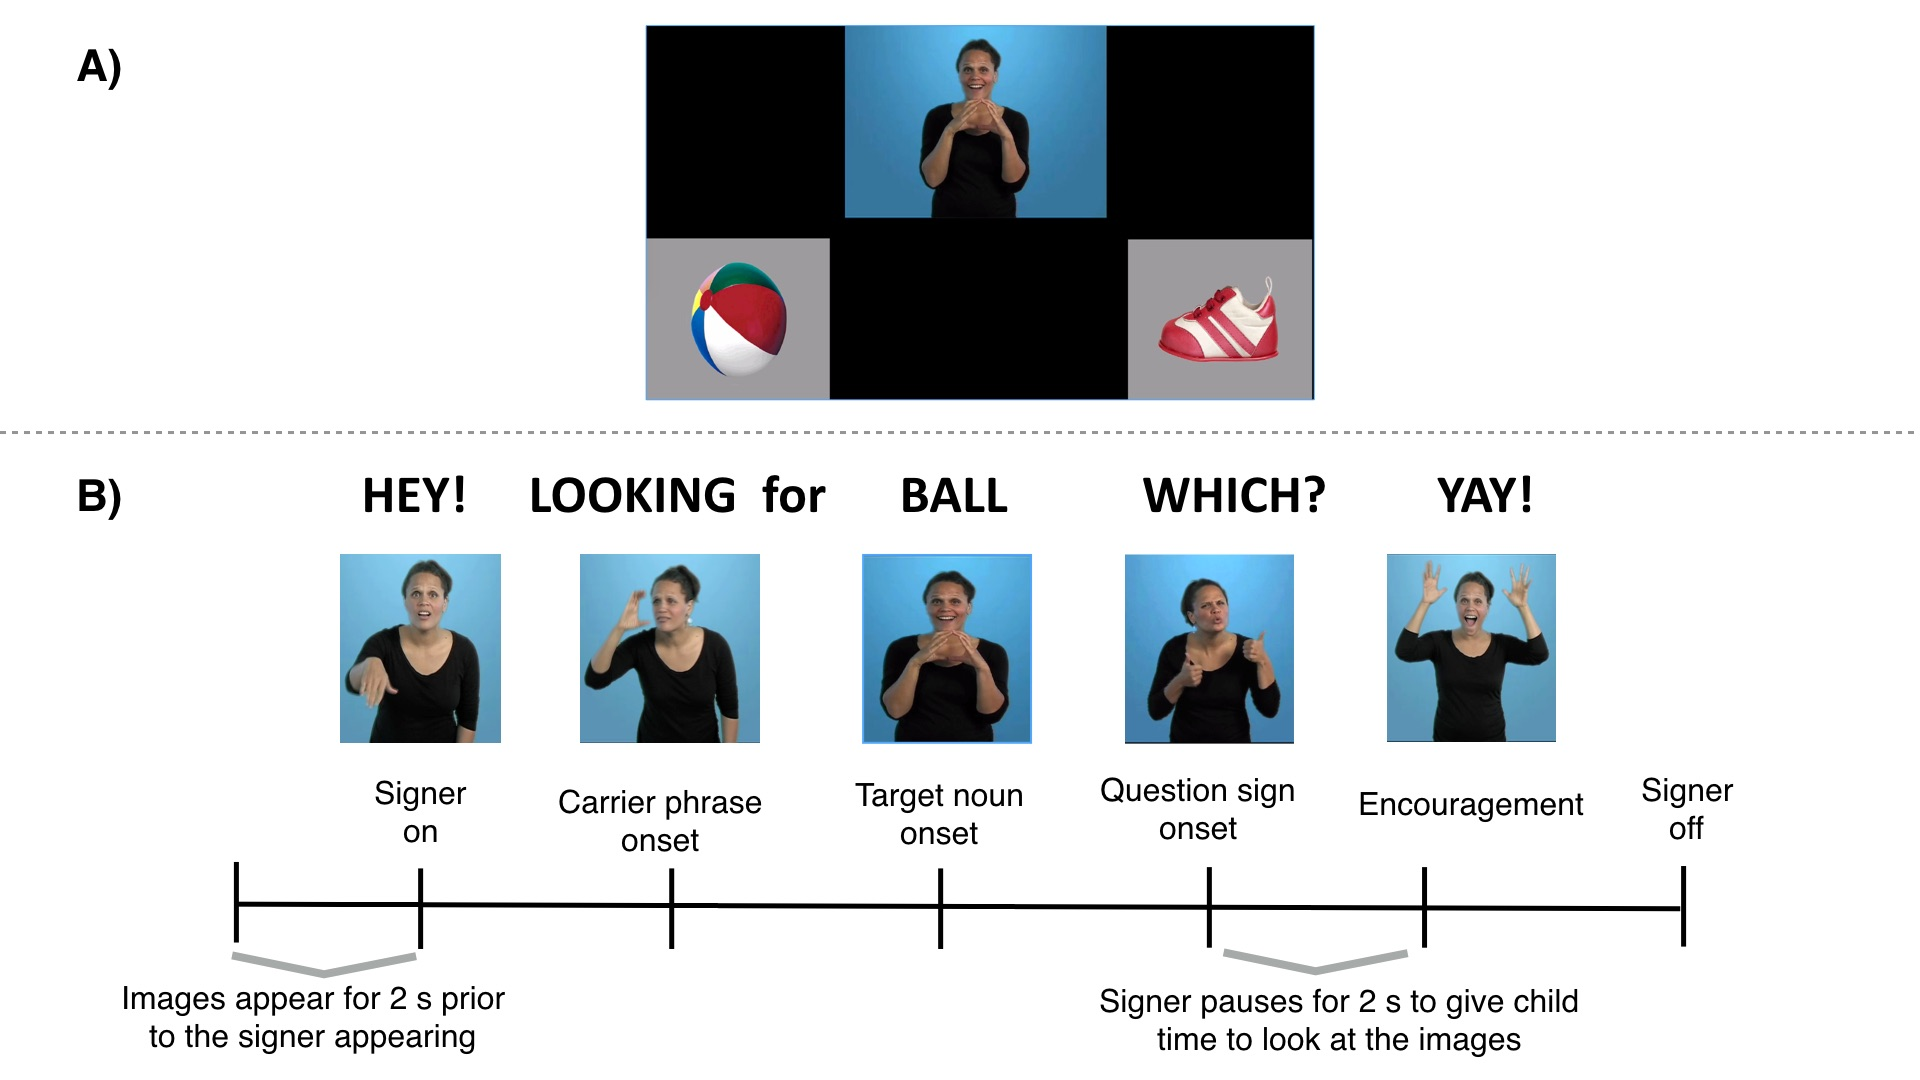
\includegraphics[width=0.95\linewidth]{/Users/kmacdonald/Documents/Projects/dissertation/index/chapter_child_rmds/SOL/figures/figure1} 

}

\caption[Stimuli in the Visual Language Processing Task]{Configuration of visual stimuli (1A) and trial structure (1B) for one question type (sentence final wh-phrase) shown in the central video on the VLP task.}\label{fig:sol-trial-fig}
\end{figure}
\hypertarget{trial-structure}{%
\subsection{Trial Structure}\label{trial-structure}}

Figure 1 shows the structure of a trial with a sentence-final wh-phrase,
one of the two question types in the VLP task. On each trial, children
saw two images of familiar objects on the screen for 2 s before the
signer appeared, allowing time for children to inspect both images.
Next, children saw a still frame of the signer for one second, so they
could orient to the signer prior to sentence onset. The target sentence
was then presented, followed by a question and 2-s hold, followed by an
exclamation to encourage attention to the task. This structure is nearly
identical to the auditory LWL task, differing only in the addition of
the 2-s hold. The hold was included to give participants additional time
to shift gaze from the signer to the objects.

\hypertarget{calculating-measures-of-language-processing-efficiency}{%
\subsection{Calculating measures of language processing
efficiency}\label{calculating-measures-of-language-processing-efficiency}}

\emph{Computing target sign onset and offset.} In studies of spoken
language processing, target word onset is typically identified as the
first moment in the auditory signal when there is acoustic evidence of
the target word. However, in signed languages like ASL, phonological
information is present in several components of the visual signal
simultaneously -- for example, in one or both hands as well as in the
face of the signer - making it difficult to determine precisely the
beginning of the target sign. Because sign onset is critical to
operationalizing speed of ASL comprehension in this task, we applied an
empirical approach to defining target-sign onset. We used a gating task
in which adult signers viewed short videos of randomly presented tokens
that varied in length. Two native signers first selected a sequence of
six candidate frames for each token, and then 10 fluent adult signers
unfamiliar with the stimuli watched videos of the target signs in
real-time while viewing the same picture pairs as in the VLP task.
Participants indicated their response with a button press. For each sign
token, the onset of the target noun was operationalized as the earliest
video frame? at which adults selected the correct picture with 100\%
agreement. To determine sign offset, two native signers independently
marked the final frame at which the handshape of each target sign was no
longer identifiable. Agreements were resolved by discussion. Sign length
was defined as sign offset minus sign onset (Median sign length was 1204
ms, ranging from 693-1980 ms).

\emph{Reaction Time.} Reaction time (RT) corresponds to the latency to
shift from the central signer to the target picture on all
signer-to-target shifts, measured from target-noun onset. We chose
cutoffs for the window of relevant responses based on the distribution
of children's RTs in the VLP task, including the middle 90\% (600-2500
ms) (see Ratcliff, 1993). Incorrect shifts (signer-to-distracter
{[}19\%{]}, signer-to-away {[}14\%{]}, no shift {[}8\%{]}) were not
included in the computation of median RT. The RT measure was reliable
within participants (Cronbach's \(\alpha = 0.8\)).

\emph{Target Accuracy.} Accuracy was the mean proportion of time spent
looking at the target picture out of the total time looking at either
target or distracter picture over the 600 to 2500 ms window from target
noun onset. We chose this window to be consistent with the choice of the
RT analysis window. This measure of accuracy reflects the tendency both
to shift quickly from the signer to the target picture in response to
the target sign and to maintain fixation on the target picture. Mean
proportion looking to target was calculated for each participant for all
trials on which the participant was fixating on the center image at
target-sign onset. To make accuracy proportion scores more suitable for
modeling on a linear scale, all analyses were based on scores that were
scaled in log space using a logistic transformation. The Accuracy
measure was reliable within participants (Cronbach's \(\alpha = 0.92\))

\emph{Proportion Sign Length Processed Prior to Shifting.} As a measure
of incremental processing, we used the mean proportion of the target
sign that children and adults saw before generating an initial eye
movement away from the central signer. Because target signs differed in
length across trials, we divided each RT value by the length of the
corresponding target sign. Previous research on spoken language suggests
that at least 200 ms is required to program an eye-movement (Salverda,
Kleinschmidt, \& Tanenhaus, 2014), so we subtracted 200 ms from each RT
to account for eye movements that were initiated during the end of the
target sign (proportion target sign =
\(\frac{(RT-200 \text{ms})}{\text{Sign Length}}\)). Mean proportion of
sign processed was computed for each token of each target sign and then
averaged over all target signs within participants, reflecting the
amount of information signers processed before generating an eye
movement, on average. A score of \(\geq\) 1.0 indicates that a signer
tended to initiate eye movements to the target pictures after sign
offset. An average \(<\) 1.0 indicates eye-movements were planned during
the target sign, reflecting the degree to which signers showed evidence
of incremental language processing.

\hypertarget{analysis-plan}{%
\subsection{Analysis Plan}\label{analysis-plan}}

We used Bayesian methods to estimate the associations between hearing
status, age, vocabulary, and RT and accuracy in the VLP task. Bayesian
methods are desirable for two reasons: First, Bayesian methods allowed
us to quantify support in favor of a null hypothesis of interest -- in
this case, the absence of a difference in real-time processing skills
between age-matched deaf and hearing ASL learners. Second, since native
ASL learners are rare, we wanted to use a statistical approach that
allowed us to incorporate relevant prior knowledge to constrain our
estimates of the strength of association between RT/accuracy on the VLP
task and age/vocabulary.

Concretely, we used prior work on the development of real-time
processing efficiency in children learning spoken language (Fernald et
al., 2008) to consider only plausible linear associations between
age/vocabulary and RT/accuracy, thus making our alternative hypotheses
more precise. In studies with adults, the common use of eye movements as
a processing measure is based on the assumption that the timing of the
first shift reflects the speed of their word recognition (Tanenhaus,
Magnuson, Dahan, \& Chambers, 2000).\footnote{The assumption that first
  shifts reflects speed of incremental word recognition depends on the
  visual display containing candidate objects with minimal initial
  phonological overlap. If there are phonological competitors present
  (e.g., candy vs.~candle), then participants' early shifting behavior
  could reflect consideration of alternative lexical hypotheses for the
  incoming linguistic information.} However, studies with children have
shown that early shifts are more likely to be random than later shifts
(Fernald et al., 2008), suggesting that some children's shifting
behavior may be unrelated to real-time ASL comprehension. We use a
mixture-model to quantify the probability that each child participant's
response is unrelated to their real-time sign recognition (i.e., that
the participant is responding randomly, or is ``guessing''), creating an
analysis model where participants who were more likely to be guessers
have less influence on the estimated relations between RT and
age/vocabulary. Note that we use this approach only in the analysis of
RT, since ``guessing behavior'' is integral to our measure of children's
mean accuracy in the VLP task, but not to our measure of mean RT. The
Supplemental Material available online provides more details about the
analysis model, as well two additional sensitivity analyses, which
provide evidence that our results are robust to different specifications
of prior distributions and to different analysis windows. We also
provide a parallel set of analyses using a non-Bayesian approach, which
resulted in comparable findings.

To provide evidence of developmental change, we report the strength of
evidence for a linear model with an intercept and slope, compared to an
intercept-only model in the form of a Bayes Factor (BF) computed via the
Savage-Dickey method (Wagenmakers et al., 2010). To estimate the
uncertainty around our estimates of the linear associations, we report
the 95\% Highest Density Interval (HDI) of the posterior distribution of
the intercept and slope. The HDI provides a range of plausible values
and gives information about the uncertainty of our point estimate of the
linear association. Models with categorical predictors were implemented
in STAN (Stan Development Team, 2016), and models with continuous
predictors were implemented in JAGS (Plummer, 2003). Finally, we chose
the linear model because it a simple model of developmental change with
only two parameters to estimate, and the outcome measures -- mean RT and
Accuracy for each participant -- were normally distributed. All of the
linear regressions include only children's data and take the form:
\(\textit{processing measure ~ age}\) and
\(\textit{processing measure ~ vocabulary}\).

\hypertarget{results}{%
\section{Results}\label{results}}

The results are presented in five sections addressing the following
central questions in this research. First, where do ASL users look while
processing sign language in real-time? Here we provide an overview of
the time course of looking behavior in our task for both adults and
children. Second, would young ASL-learners and adult signers show
evidence of rapid gaze shifts that reflect lexical processing, despite
the apparent competition for visual attention between the language
source and the nonlinguistic visual world? In this section, we estimate
the degree to which children and adults tended to initiate eye-movements
prior to target sign offset, providing evidence that these gaze shifts
occur prior to sign offset and index speed of incremental ASL
comprehension. Third, do deaf and hearing native signers show a similar
time course of eye movements, despite having differential access to
auditory information in their daily lives? Or would deaf children's
daily experience relying on vision to monitor both the linguistic signal
and the potential referents in the visual world result in a
qualitatively different pattern of performance, e.g., their waiting
longer to disengage from the signer to seek the named object? Fourth, do
young ASL-learners show age-related increases in processing efficiency
that parallel those found in spoken languages? Here we compare
ASL-learners' processing skills to those of adult signers and exploring
relations to age among the children. Finally, is individual variation in
children's ASL processing efficiency related to the size of their
productive ASL vocabularies?
\begin{figure}[t]

{\centering 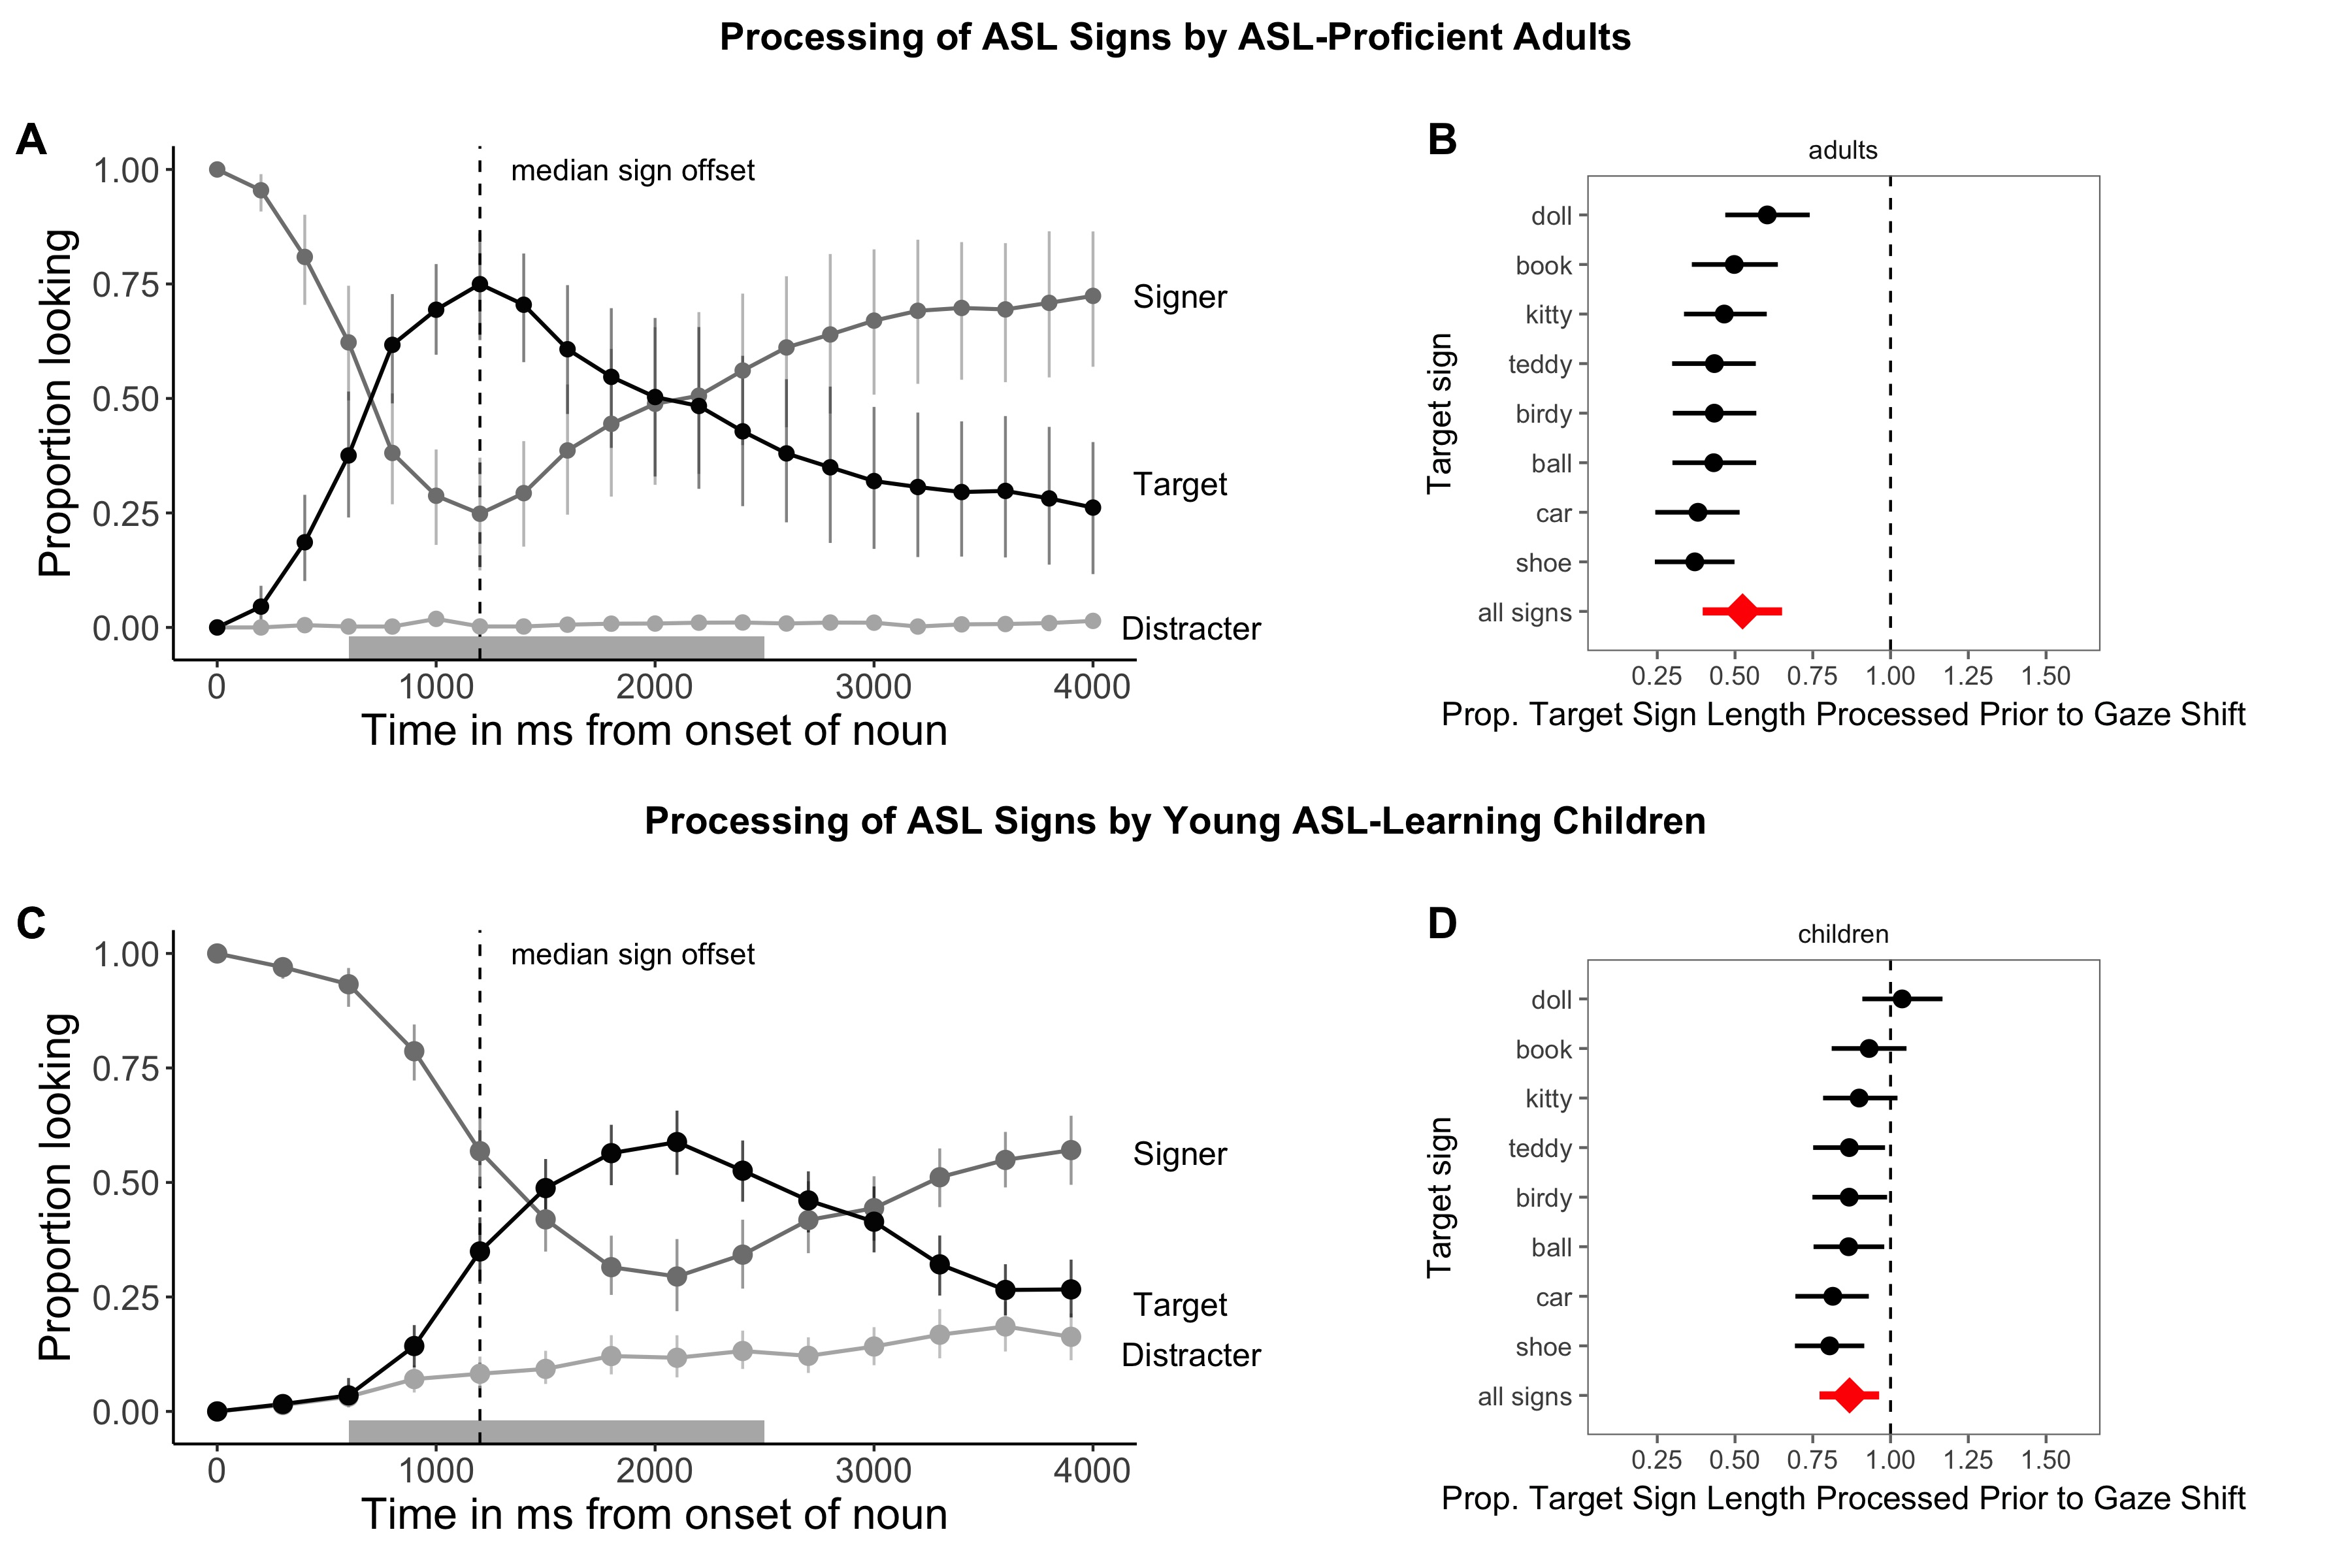
\includegraphics[width=0.95\linewidth]{/Users/kmacdonald/Documents/Projects/dissertation/index/chapter_child_rmds/SOL/figures/figure2} 

}

\caption[Time course looking behavior for ASL-proficient adults and young ASL-learners]{The time course of looking behavior for ASL-proficient adults (2A) and young ASL-learners (2C). The curves show mean proportion looking to the signer (dark grey), the target image (black), and the distracter image (light grey). The grey shaded region marks the analysis window (600-2500ms); error bars represent +/- 95\% CI computed by non-parametric bootstrap. The mean proportion of each target sign length (see the Methods section for details on how sign length was defined) processed prior to shifting visual attention away from the language source to a named object for adults (2B) and children (2D). The diamond indicates the mean estimate for all signs. The dashed vertical line corresponds to a median proportion of 1.0. Error bars represent 95\% Highest Density Intervals.}\label{fig:sol-tc-figure}
\end{figure}
\hypertarget{overview-of-looking-behavior-during-real-time-asl-comprehension}{%
\subsection{Overview of looking behavior during real-time ASL
comprehension}\label{overview-of-looking-behavior-during-real-time-asl-comprehension}}

The first question of interest was where do ASL users look while
processing sign language in real-time? Figure 2 presents an overview of
adults (2A) and children's (2B) looking behavior in the VLP task. This
plot shows changes in the mean proportion of trials on which
participants fixated the signer, the target image, or the distracter
image at every 33-ms interval of the stimulus sentence. At target-sign
onset, all participants were looking at the signer on all trials. As the
target sign unfolded, the mean proportion looking to the signer
decreased rapidly as participants shifted their gaze to the target or
the distracter image. Proportion looking to the target increased sooner
and reached a higher asymptote, compared to proportion looking to the
distracter, for both adults and children. After looking to the target
image, participants tended to shift their gaze rapidly back to the
signer, shown by the increase in proportion looking to the signer around
2000 ms after target-noun onset. Adults tended to shift to the target
picture sooner in the sentence than did children, and well before the
average offset of the target sign. Moreover, adults rarely looked to the
distractor image at any point in the trial. This systematic pattern of
behavior -- participants reliably shifting attention from the signer to
the named object and back to the signer -- provides qualitative evidence
that the VLP task is able to capture interpretable eye movement behavior
during ASL comprehension.

\hypertarget{evidence-that-eye-movements-during-asl-processing-index-incremental-sign-comprehension}{%
\subsection{Evidence that eye movements during ASL processing index
incremental sign
comprehension}\label{evidence-that-eye-movements-during-asl-processing-index-incremental-sign-comprehension}}

One of the behavioral signatures of proficient spoken language
processing is the rapid influence of language on visual attention, with
eye movements occurring soon after listeners have enough information to
identify the named object. Our second question of interest was whether
young ASL-learners and adult signers would also show evidence of rapid
gaze shifts in response to signed language, despite the apparent
competition for visual attention between the language source and the
nonlinguistic visual world. Or would signers delay their shifts until
the very end of the target sign, or even until the end of the utterance,
perhaps because they did not want to miss subsequent linguistic
information?

To answer these questions, we conducted an exploratory analysis,
computing the proportion of each target sign that participants processed
before generating an eye movement to the named object. Figure 2 shows
this measure for each target sign for both adults (2B) and children
(2D). Adults shifted prior to the offset of the target sign for all
items and processed on average 51\% of the target sign before generating
a response (M = 0.51, 95\% HDI {[}0.35, 0.66{]}). Children processed
88\% of the target sign on average, requiring more information before
shifting their gaze compared to adults. Children reliably initiated
saccades prior to the offset of the target sign overall (M = 0.88, 95\%
HDI {[}0.79, 0.98{]}) and for five out of the eight signed stimuli.

These results suggest that young signers as well as adults process signs
incrementally as they unfold in time (for converging evidence see
Lieberman et al., 2015, 2017). It is important to point out that we
would not interpret signers waiting until the end of the sign or the end
of the sentence as evidence against an incremental processing account
since there could be other explanations for that pattern of results such
as social norms of looking at a person until they finish speaking.
However, this result provides positive evidence that eye movements in
the VLP task provide an index of speed of incremental ASL comprehension,
allowing us to perform the subsequent analyses that estimate (a) group
differences in looking behavior and (b) links between individual
variation in speed and accuracy of eye movements during ASL processing
and variation in productive vocabulary.
\begin{figure}[t]

{\centering 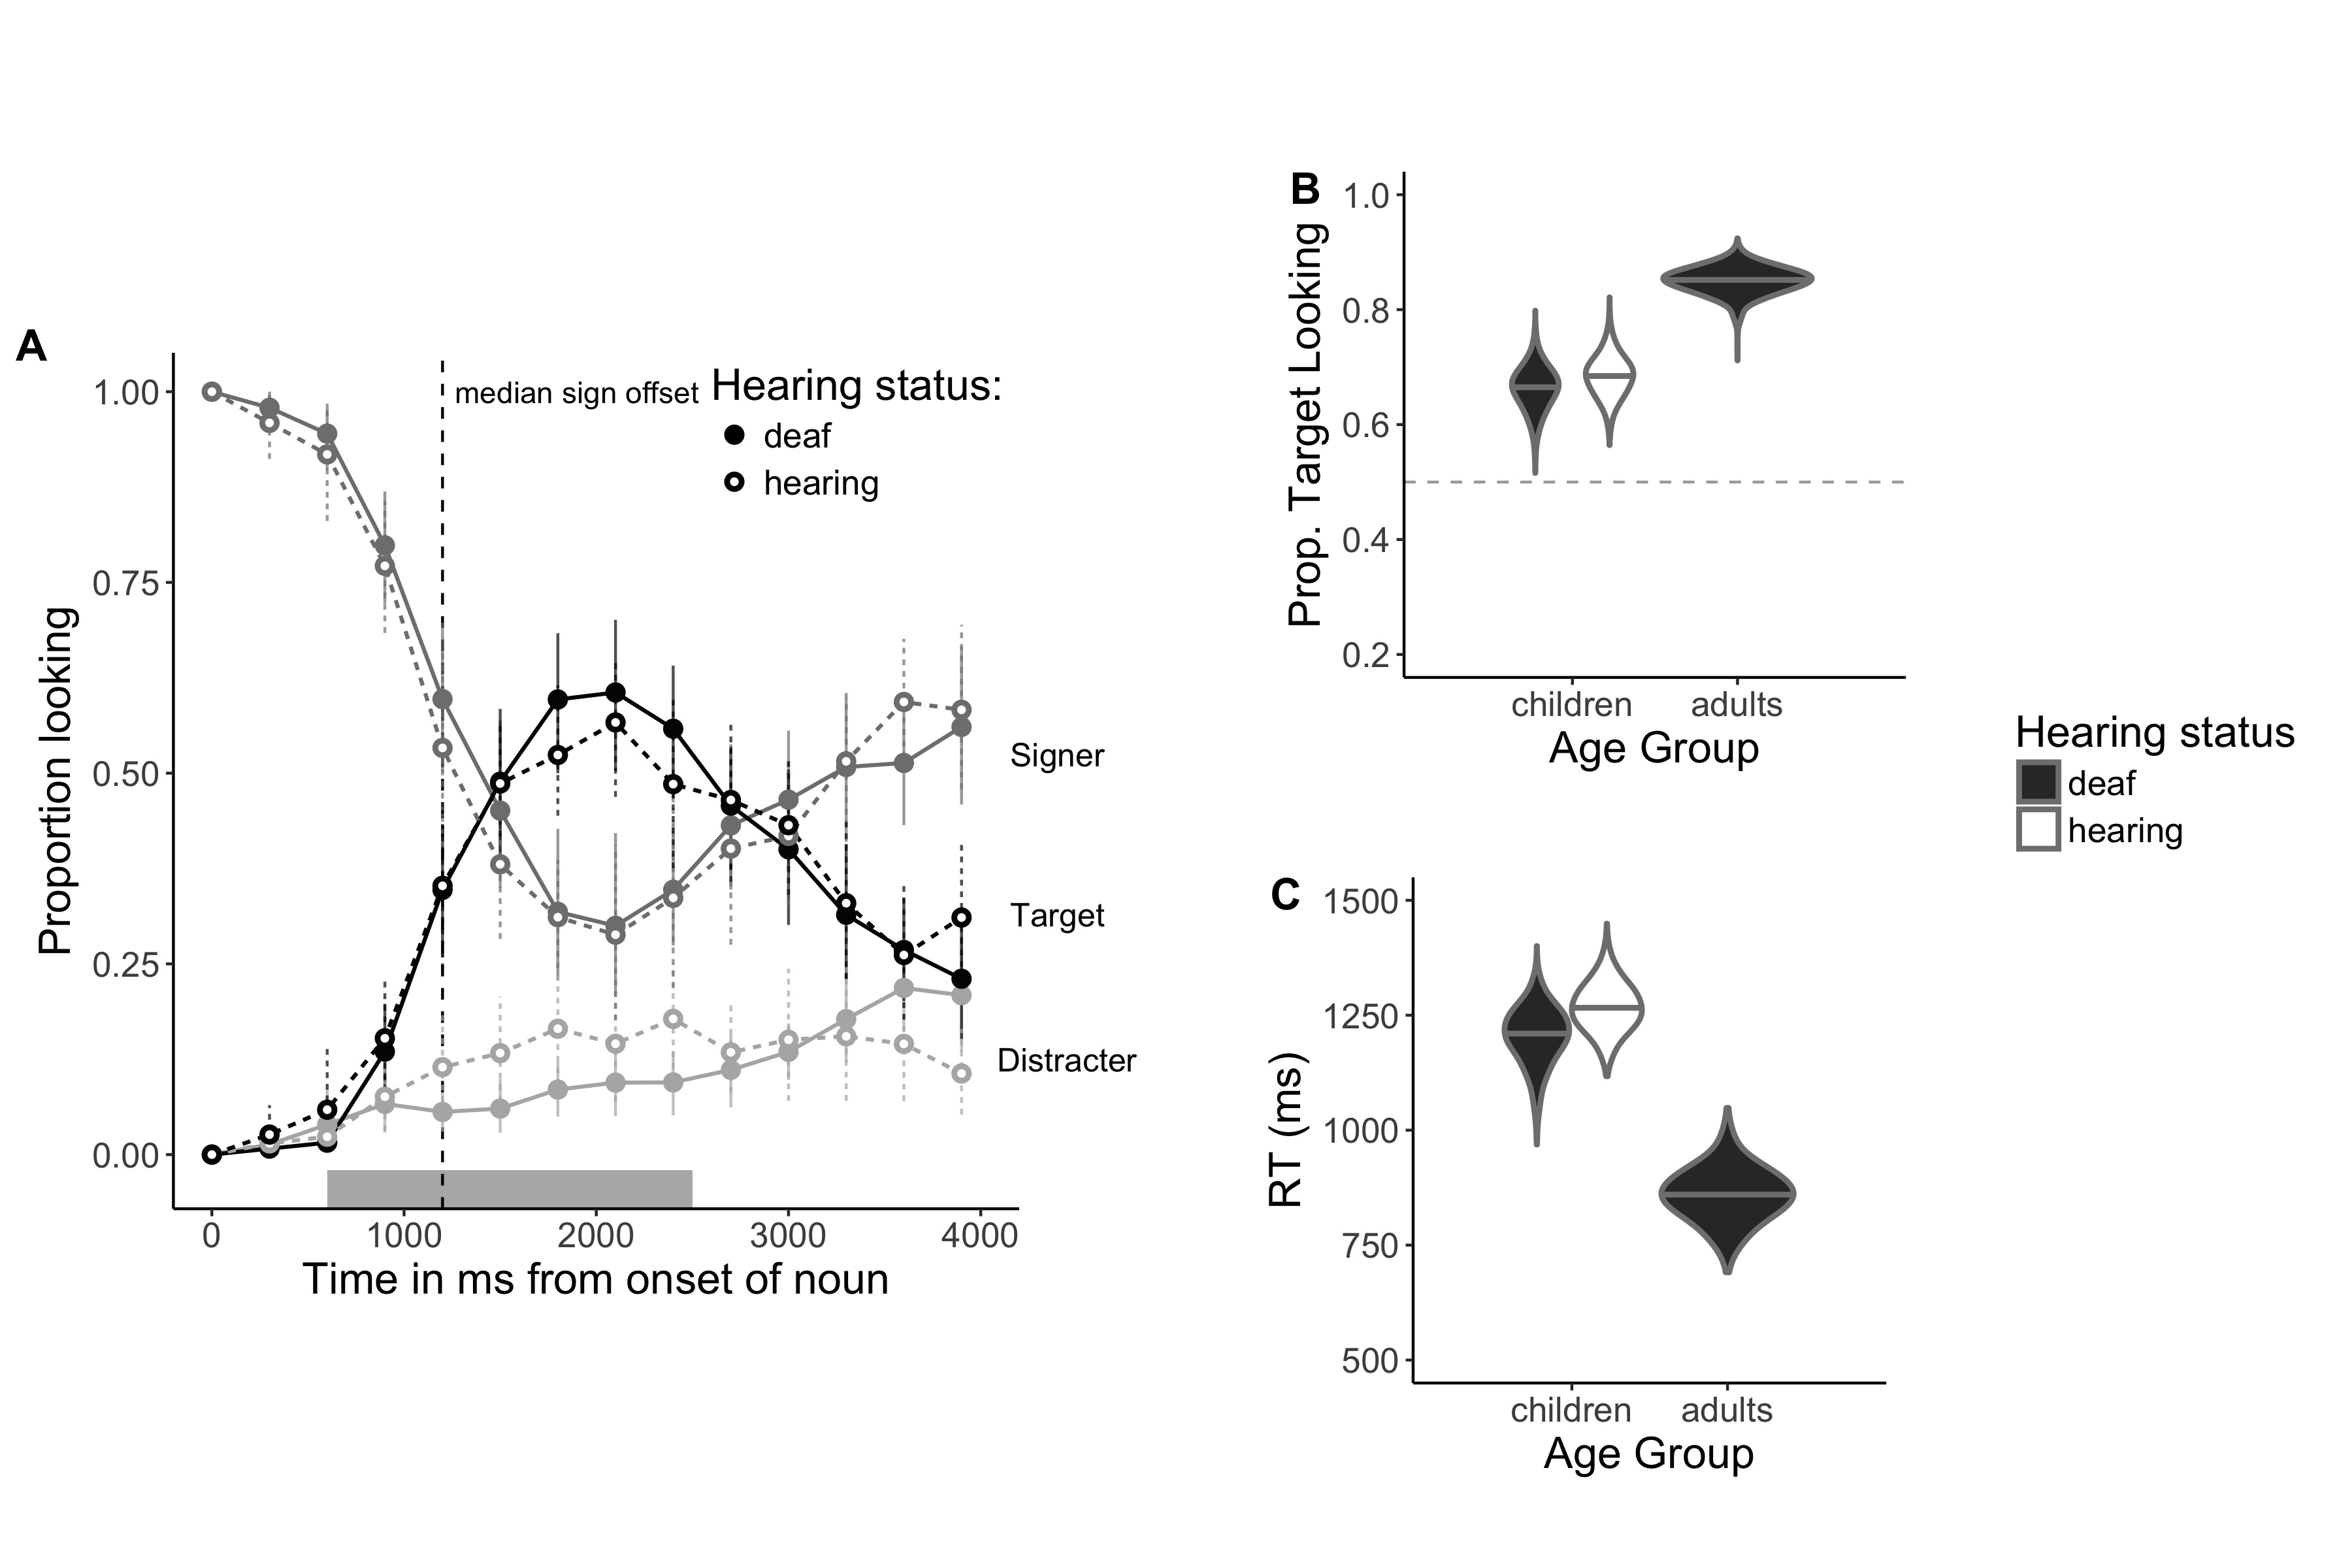
\includegraphics[width=0.95\linewidth]{/Users/kmacdonald/Documents/Projects/dissertation/index/chapter_child_rmds/SOL/figures/figure3} 

}

\caption[The time course of looking behavior for young deaf and hearing ASL-learners]{The time course of looking behavior for young deaf and hearing ASL-learners (3A). Filled circles represent deaf signers, while open circles represent hearing signers; All other plotting conventions are the same as in Figure 2. Panels B and C show full posterior distributions over model estimates for mean Accuracy (3B) and Reaction Time (3C) for children and adults. Fill (white/black) represents children's hearing status. (Note that there were no hearing adult signers in our sample).}\label{fig:sol-tc-coda-figure}
\end{figure}
\hypertarget{real-time-asl-comprehension-in-deaf-and-hearing-children-and-deaf-adults}{%
\subsection{Real-time ASL comprehension in deaf and hearing children and
deaf
adults}\label{real-time-asl-comprehension-in-deaf-and-hearing-children-and-deaf-adults}}

The third question of interest was whether deaf and hearing native
signers show a similar time course of lexical processing, driven by
their similar language experiences and the in-the-moment constraints of
interpreting a sign language in real time? Or would deaf children's
daily experience relying on vision to monitor both the linguistic signal
and the potential referents in the visual world result in a
qualitatively different pattern of performance, e.g., their waiting
longer to disengage from the signer to seek the named object?

Figure 3A presents the overview of looking behavior for deaf and hearing
children. At target-sign onset, all children were looking at the signer
on all trials. Overall, deaf and hearing children showed a remarkably
similar time course of looking behavior: shifting away from the signer,
increasing looks to the target, and shifting back to the signer at
similar time points as the sign unfolded. To quantify any differences,
we compared the posterior distributions for mean accuracy (Figure 3B)
and mean RT (Figure 3C) across the deaf and hearing groups. We did not
find evidence for a difference in mean accuracy (M\_(hearing) 〖=0.68,〖
M〗\emph{(deaf= ) 0.65; β〗\emph{diff= 0.03, 95\% HDI {[}-0.07, 0.13{]})
or RT 〖(M〗}(hearing) 〖=1265.62 ms,〖 M〗}(deaf= ) 1185.05 ms;
β〗\_diff= 78.32 ms, 95\% HDI {[}-86.01 ms, 247.04 ms{]}), with the 95\%
HDI including zero for both models. These parallel results provide
evidence that same-aged hearing and deaf native ASL-learners showed
qualitatively similar looking behavior during real-time sentence
processing, suggesting that decisions about where to allocate visual
attention are not modulated by differential access to auditory
information, but rather are shaped by learning ASL as a first language
(see Bavelier et al., 2006 for a review of the differential effects of
deafness compared to learning a visual language on perception and
higher-order cognitive skills). Moreover, these results provide
additional justification (over and above children's highly similar
language background experience) for analyzing all the native
ASL-learning children together, regardless of hearing status, in the
subsequent analyses.

Returning to the overview of looking behavior shown in Figure 2, we see
that adults tended to shift to the target picture sooner in the sentence
than did children, and well before the average offset of the target
sign. Moreover, adults rarely looked to the distractor image at any
point in the trial. To quantify these age-related differences we
computed the full posterior distribution for children and adults' mean
Accuracy (Figure 3B) and RT (Figure 3C). Overall, adults were more
accurate (M\_adults= 0.85, M\_(children)= 0.68, β\_diff = 0.17, 95\% HDI
for the difference in means {[}0.11, 0.24{]}) and faster to shift to the
target image compared to children (M\_adults= 861.98 ms, M\_(children)=
1229.95 ms; β\_diff = -367.76 ms, 95\% HDI for the difference in means
{[}-503.42 ms, -223.85 ms{]}). This age-related difference parallels
findings in spoken language (Fernald et. al., 2006) and shows that young
ASL learners are still making progress towards adult-levels of ASL
processing efficiency.
\begin{figure}[t]

{\centering 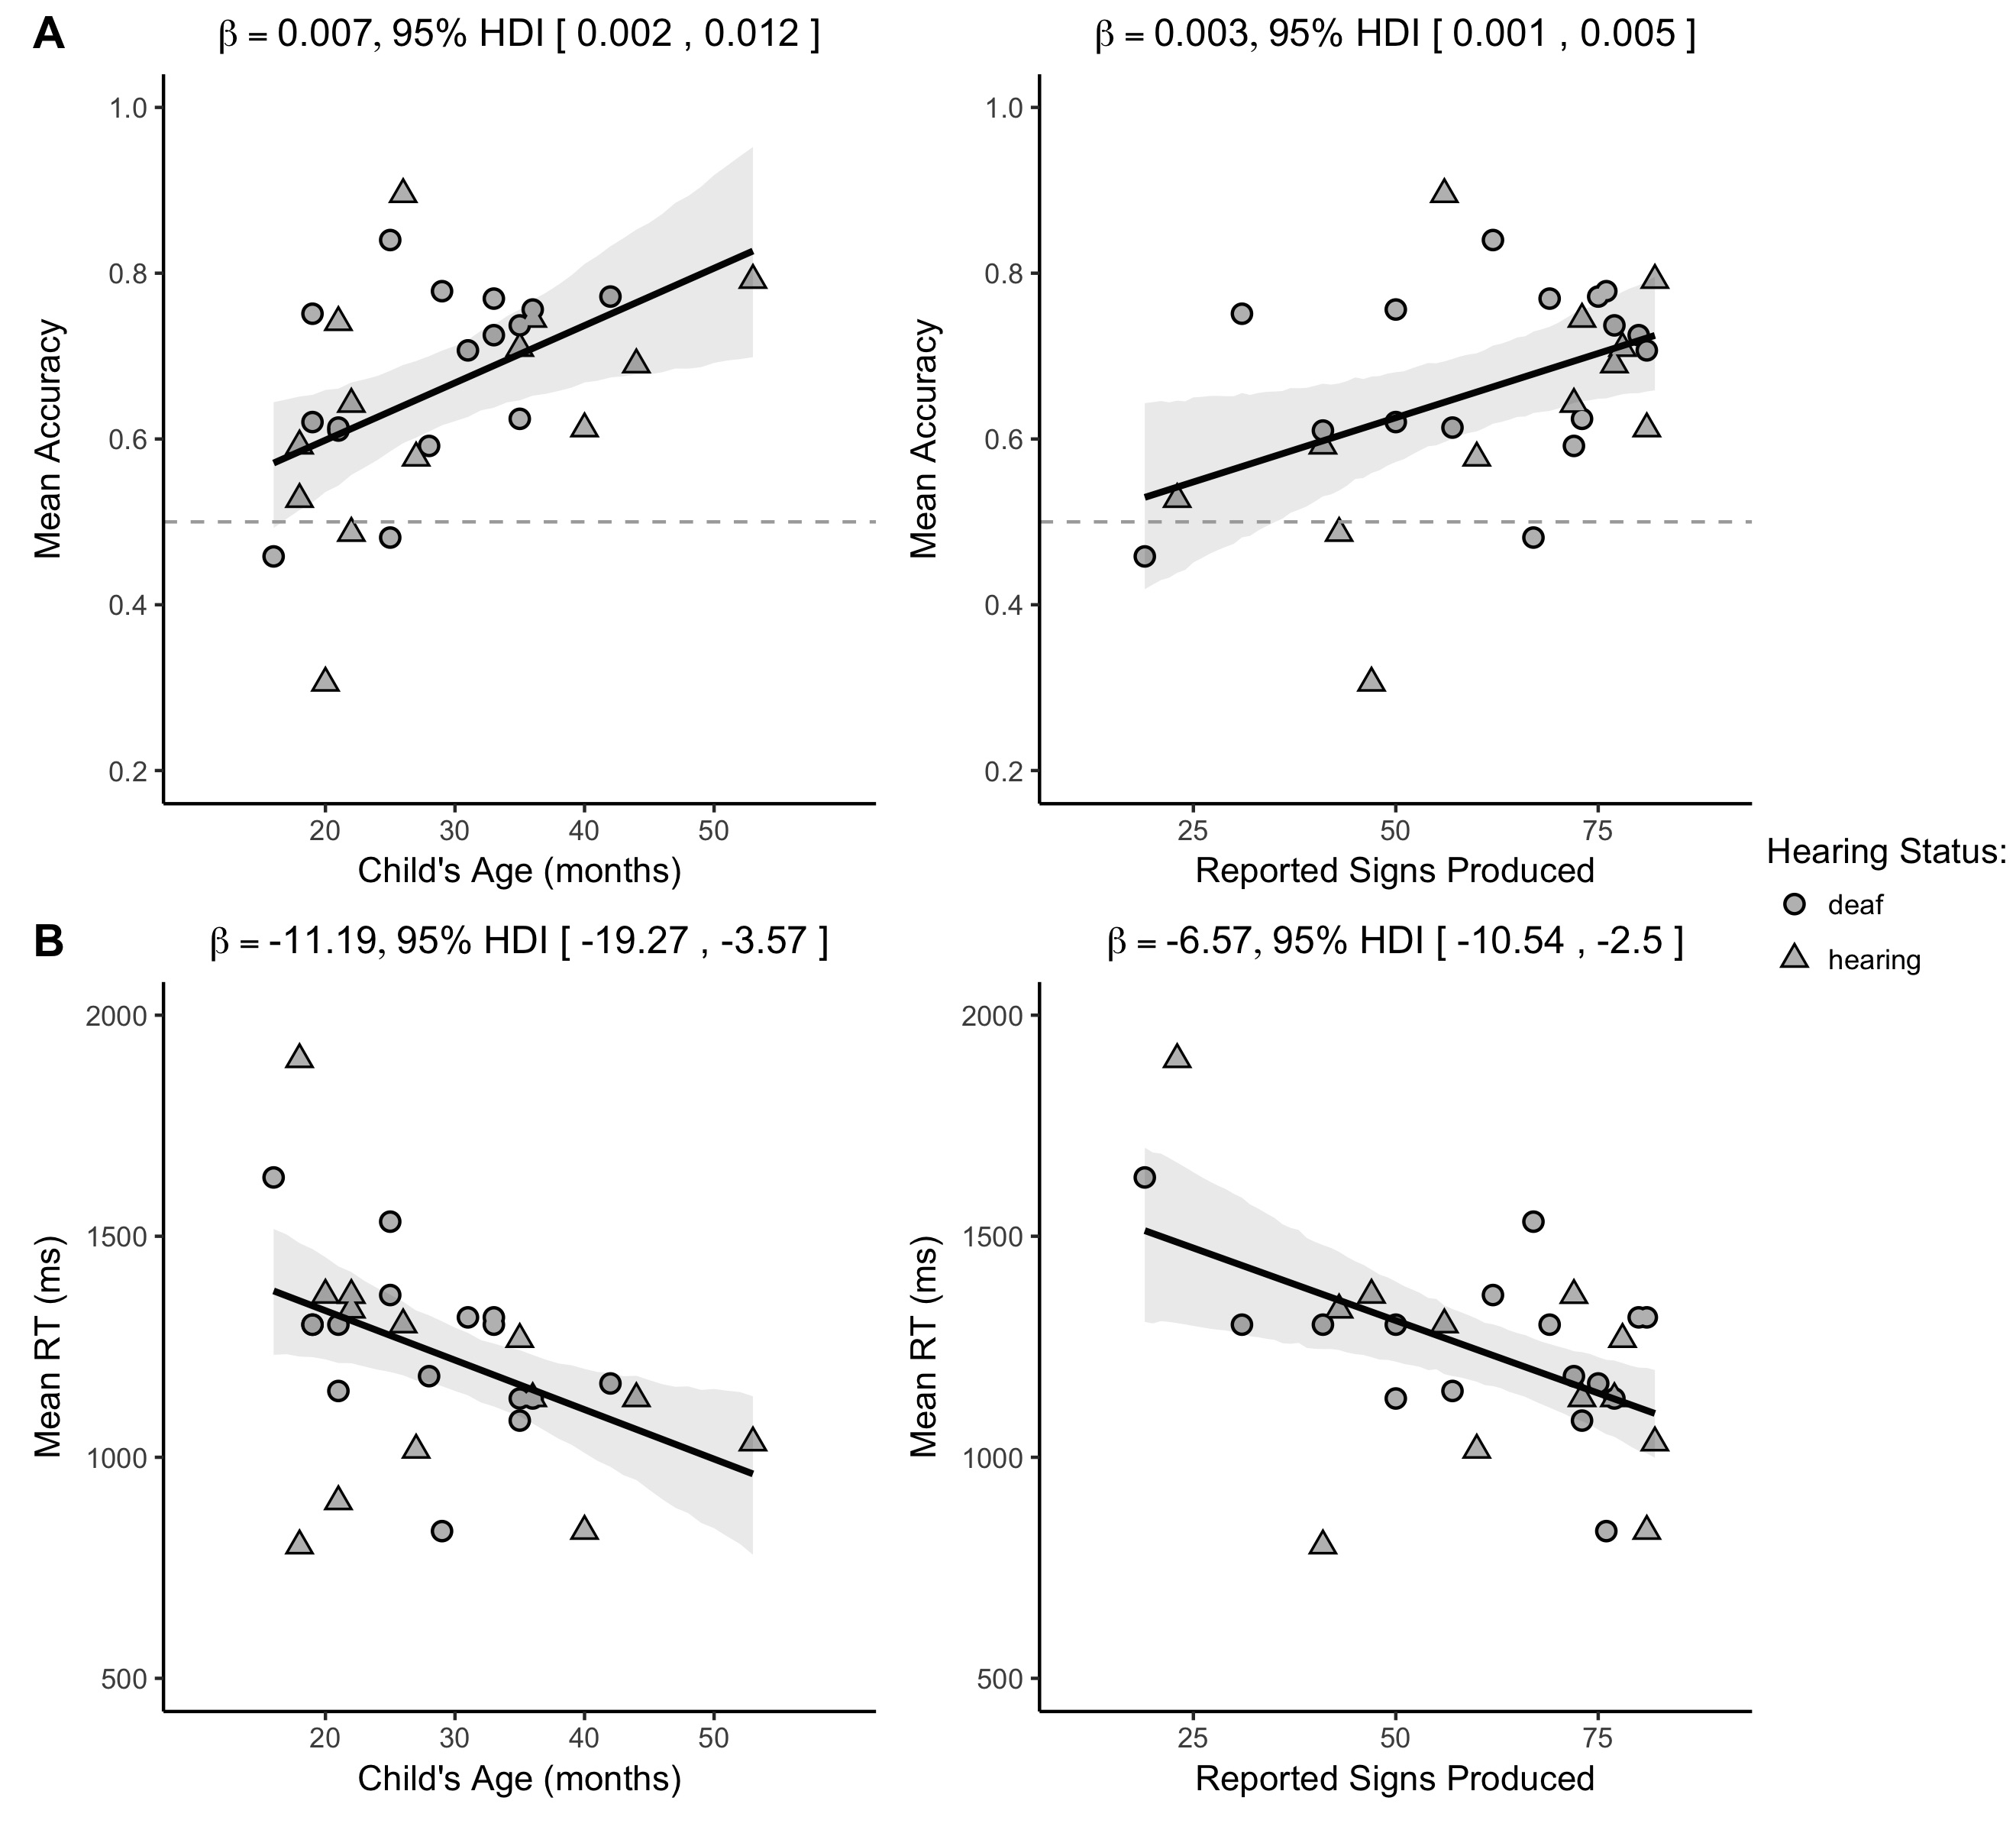
\includegraphics[width=0.8\linewidth]{/Users/kmacdonald/Documents/Projects/dissertation/index/chapter_child_rmds/SOL/figures/figure4} 

}

\caption[Scatterplots of relations between children's age and vocabulary and ASL processing]{Scatterplots of relations between children's age and vocabulary and measures of their mean accuracy (4A) and mean RT (4B) in the VLP procedure. Shape represents children's hearing status. The solid black line is the maximum a posteriori model estimate for the mean accuracy at each age point. The shaded gray regions represent the 95\% Highest Density Interval (range of plausible values) around the regression line.}\label{fig:sol-corr-figure}
\end{figure}
Next, we compared real-time processing efficiency in ASL-learners and
adult signers. Returning to the overview of looking behavior shown in
Figure 2, we see that adults tended to shift to the target picture
sooner in the sentence than did children, and well before the average
offset of the target sign. Moreover, adults rarely looked to the
distractor image at any point in the trial. To quantify these
differences we computed the full posterior distribution for children and
adults' mean Accuracy (Figure 3B) and RT (Figure 3C). Overall, adults
were more accurate (M\_adults= 0.85, M\_(children)= 0.68, β\_diff =
0.17, 95\% HDI for the difference in means {[}0.11, 0.24{]}) and faster
to shift to the target image compared to children (M\_adults= 861.98 ms,
M\_(children)= 1229.95 ms; β\_diff = -367.76 ms, 95\% HDI for the
difference in means {[}-503.42 ms, -223.85 ms{]}). This age-related
difference parallels findings in spoken language (Fernald et. al., 2006)
and shows that young ASL learners are still making progress towards
adult-levels of ASL processing efficiency.

\hypertarget{links-between-childrens-age-and-efficiency-in-incremental-sign-comprehension}{%
\subsection{Links between children's age and efficiency in incremental
sign
comprehension}\label{links-between-childrens-age-and-efficiency-in-incremental-sign-comprehension}}

The fourth question of interest was whether young ASL-learners show
age-related increases in processing efficiency that parallel those found
in spoken languages. To answer this question, we estimated relations
between young ASL learners' age-related increases in the speed and
accuracy with which they interpreted familiar signs (see Table 3 for
point and interval estimates). Mean accuracy was positively associated
with age (Figure 4A), indicating that older ASL learners were more
accurate than younger children in fixating the target picture. The Bayes
Factor (BF) indicated that a model including a linear association was
12.8 times more likely than an intercept-only model, providing strong
evidence for developmental change. The β estimate indicates that, for
each month of age, children increased their accuracy score by 0.007,
i.e., an increase of \textasciitilde{}1\% point, meaning that over the
course of one year the model estimates a \textasciitilde{}12\% point
gain in accuracy when establishing reference in the VLP task. Mean RTs
were negatively associated with age (Figure 4A), indicating that older
children shifted to the target picture more quickly than did younger
children. The BF was \textasciitilde{}14, providing strong evidence for
a linear association. The model estimates a \textasciitilde{}11 ms gain
in RT for each month, leading to a \textasciitilde{}132 ms gain in speed
of incremental ASL comprehension over one year of development.

Together, the accuracy and RT analyses showed that young ASL learners
reliably looked away from the central signer to shift to the named
target image in the VLP task. Importantly, children varied in their
response times and accuracy, and this variation was meaningfully linked
to age. Thus, like children learning spoken language, ASL learners
improve their real-time language processing skills over the second and
third years of life as they make progress towards adult levels of
language fluency.
\begin{longtable}[t]{>{\raggedright\arraybackslash}p{4cm}rll}
\caption[Summary of the four linear models using children's age and vocabulary size to predict accuracy and reaction time]{\label{tab:sol-bf-table}Summary of the four linear models using children's age and vocabulary size to predict accuracy (proportion looking to target) and reaction time (latency to first shift in ms). BF is the Bayes Factor comparing the evidence in favor of linear model to an intercept-only (null) model; Mean Beta is the mean of the posterior distribution for the slope parameter for each model (i.e., the linear association); and the Highest Density Interval (HDI) shows the interval containing 95\% of the plausible slope values given the model and the data.}\\
\toprule
\textbf{Model specification} & \textbf{Bayes Factor} & \textbf{Mean Beta} & \textbf{95\% HDI}\\
\midrule
Accuracy \textasciitilde{} Age & 12.8 & 0.007 & [0.002, 0.012]\\
Accuracy \textasciitilde{} Vocab & 6.8 & 0.003 & [0.001, 0.005]\\
RT \textasciitilde{} Age & 14.4 & -11.2 ms & [-19.3 ms, -3.6 ms]\\
RT \textasciitilde{} Vocab & 18.7 & -6.6 ms & [-10.5 ms, -2.5 ms]\\
\bottomrule
\end{longtable}
\hypertarget{links-between-childrens-incremental-sign-comprehension-and-productive-vocabulary}{%
\subsection{Links between children's incremental sign comprehension and
productive
vocabulary}\label{links-between-childrens-incremental-sign-comprehension-and-productive-vocabulary}}

The final question of interest was whether individual differences in
processing skills were related to the size of children's ASL
vocabularies. As shown in Figure 4B, children with higher accuracy
scores also had larger productive vocabularies (BF = 6.8), with the
model estimating a 0.003 increase for each additional sign known.
Moreover, children who were faster to recognize ASL signs were those
with larger sign vocabularies (BF = 18.7), with each additional sign
resulting in a \textasciitilde{}7 ms decrease in estimated RT. Taken
together, older children and children with larger expressive
vocabularies were more accurate and efficient in identifying the
referents of familiar signs. It is important to point out that the
independent effect of vocabulary size on ASL processing could not be
assessed here given the correlation between age and vocabulary (r =
0.76) in our sample of children ages one to four years. However, these
findings parallel results in the substantial body of previous research
with monolingual children learning spoken languages, such as English
(Fernald et al., 2006) and Spanish (Hurtado, Marchman, \& Fernald,
2007).

\hypertarget{discussion}{%
\section{Discussion}\label{discussion}}

Efficiency in establishing reference in real-time lexical processing is
a fundamental component of language learning. Here, we developed the
first measures of young ASL learners' real-time language comprehension
skills. There are five main findings from this research.

First, both adults and children showed a similar qualitative pattern of
looking behavior as signs unfolded in time. They began by looking at the
signer to gather information about the signed sentence, before shifting
gaze to the named object, followed by a return in looking to the signer.
All signers allocated very few fixations to the distractor image at any
point during the signed sentence.

Second, children and adults tended to shift their gaze away from the
signer and to the named referent prior to sign offset, providing
evidence of incremental ASL processing. This rapid influence of language
on visual attention in ASL is perhaps even more striking since premature
gaze shifts could result in a degraded the linguistic signal processed
in the periphery or in missing subsequent linguistic information
altogether. Furthermore, evidence of incremental gaze shifts suggests
that eye movements during ASL processing index efficiency of lexical
comprehension, as previously shown in spoken languages, which is
important for future work on the psycholinguistics of early sign
language acquisition.

Third, deaf and hearing native signers, despite having differential
access to auditory information, showed remarkably similar looking
behavior during real-time ASL comprehension. Even though the deaf and
hearing children had differential access to auditory information in
their daily lives, this experience did not change their overall looking
behavior or the timing of their gaze shifts during ASL comprehension.
Instead, both groups showed parallel sensitivity to the in-the-moment
constraints of processing ASL in real time. That is, both deaf and
hearing children allocated similar amounts of visual attention to the
signer, presumably because this was the only fixation point in the
visual scene that also provided information with respect to their goal
of language comprehension. This is in stark contrast to what hearing
children could potentially do in a similar grounded language
comprehension task where a speaker was a potential visual target. In
that case, the hearing listener could choose to look at the speaker or
to look elsewhere, without losing access to the incoming language via
the auditory channel. Thus, they can look while they listen.

Fourth, like children learning spoken language, young ASL-learners were
less efficient than adults in their real-time language processing, but
they showed significant improvement with age over the first four years.
Moreover, although all target signs were familiar to children, older
children identified the named referents more quickly and accurately than
younger children. This result suggests that the real-time comprehension
skills of children who are learning ASL in native contexts follow a
similar developmental path to that of spoken language learners, as has
been shown in previous work on ASL production (Lillo-Martin, 1999;
Mayberry \& Squires, 2006). By developing precise measures of real-time
ASL comprehension, we were able to study children's language skills
earlier in development as compared to other methods.

Fifth, we found a link between ASL processing skills and children's
productive vocabularies. ASL-learning children who knew more signs were
also faster and more accurate to identify the correct referent than
those who were lexically less advanced. These results are consistent
with studies of English- and Spanish-learning children, which find
strong relations between efficiency in online language comprehension and
measures of linguistic achievement (Fernald et al., 2006; Marchman \&
Fernald, 2008).

\hypertarget{limitations-and-open-questions}{%
\subsection{Limitations and open
questions}\label{limitations-and-open-questions}}

This study has several limitations. First, while the sample size is
larger than in most previous studies of ASL development, it is still
relatively small compared to many studies of spoken language acquisition
- an unsurprising limitation, given that native ASL-learners are a rare
population. Thus more data are needed to characterize more precisely the
developmental trajectories of sign language processing skills. Second,
testing children within a narrower age range might have revealed
independent effects of vocabulary size on ASL processing, which could
not be assessed here given the correlation between age and vocabulary
size in our broad sample of children from one to four years. To
facilitate replication and extension of our results, we have made all of
our stimuli, data, and analysis code publicly available
(\url{https://github.com/kemacdonald/SOL}).

Third, we did not collect measures of age-related gains in children's
general cognitive abilities. Thus, it is possible that our estimates of
age-related changes in lexical processing are influenced by children's
developing efficiency in other aspects of cognition, e.g., increased
control of visual attention. Work on the development of visual attention
from adolescence to early adulthood shows that different components of
visual attention (the ability to distribute attention across the visual
field, attentional recovery from distraction, and multiple object
processing) develop at different rates (Dye and Bavelier, 2009).
Moreover, work by Elsabbagh et. al., (2013) shows that infants become
more efficient in their ability to disengage from a central stimulus to
attend to a stimulus in the periphery between the ages 7 months and 14
months. However, there is a large body of work showing that features of
language use and structure (e.g., the frequency of a word, a word's
neighborhood density, and the amount of language input a child
experiences) affect the speed and accuracy of eye movements in the
Looking-While-Listening style tasks (see Tanenhaus et al., 2000 for a
review). Thus, while it possible that age-related improvements in
general cognitive abilities are a factor in our results, we think that
the strength of the prior evidence suggests that more efficient gaze
shifts in the VLP task are indexing improvements in the efficiency of
incremental ASL comprehension.

A fourth limitation is that characteristics of our task make it
difficult to directly compare our findings with previous work on ASL
processing by adults. For example, in contrast to prior gating studies
(e.g., Emmorey \& Corina, 1990; Morford \& Carlsen, 2011), our stimuli
consisted of full sentences in a child-directed register, not isolated
signs, and we used a temporal response measure rather than an open-ended
untimed response. However, it is interesting to note that the mean
reaction time of the adults in our task (M = 862 ms) is strikingly close
to the average performance of native adult signers in Lieberman et al.'s
(2015) ``unrelated'' condition (M = 844 ms). In addition, we did not
select stimuli that parametrically varied features of signs that may
influence speed of incremental ASL comprehension, including iconicity
and degree of phonological overlap. However, we were able to use a
recently created database of lexical and phonological properties of 1000
signs (Caselli et. al., 2017) to explore this possibility. We did not
see evidence that iconicity or degree of phonological overlap influenced
speed or accuracy of eye movements in children or adults in our sample
of eight target signs (see Figures S4 and S5 in the online supplement).

We also cannot yet make strong claims about processing in signed
vs.~spoken languages in absolute terms because the VLP task included the
signer as a central fixation, resulting in different task demands
compared to the two-alternative procedure used to study children's
spoken language processing (e.g., Fernald et al.~1998). However, a
direct comparison of the timecourse of eye movements during signed and
spoken language processing is a focus of our ongoing work (MacDonald et
al., 2017). Nevertheless, the current results reveal parallels with
previous findings showing incremental processing during real-time spoken
language comprehension (see Tanenhaus et al., 2000) and sign language
comprehension in adults (Lieberman et al., 2015). Moreover, we
established links between early processing efficiency and measures of
vocabulary in young ASL-learners, suggesting that parallel mechanisms
drive language development, regardless of the language modality.

Finally, our sample is not representative of most children learning ASL
in the United States. Since most deaf children are born to hearing
parents unfamiliar with ASL, many are exposed quite inconsistently to
sign language, if at all. We took care to include only children exposed
to ASL from birth. The development of real-time ASL processing may look
different in children who have inconsistent or late exposure to ASL
(Mayberry, 2007). An important step is to explore how variation in ASL
processing is influenced by early experience with signed languages.
Since children's efficiency in interpreting spoken language is linked to
the quantity and quality of the speech that they hear (Hurtado,
Marchman, \& Fernald, 2008; Weisleder \& Fernald, 2013), we would expect
similar relations between language input and outcomes in ASL-learners.
We hope that the VLP task will provide a useful method to track
precisely the developmental trajectories of a variety of ASL-learners.

\hypertarget{conclusion}{%
\section{Conclusion}\label{conclusion}}

This study provides evidence that both child and adult signers rapidly
shift visual attention as signs unfold in time and prior to sign offset
during real-time sign comprehension. In addition, individual variation
in speed of lexical processing in child signers is meaningfully linked
to age and vocabulary. These results contribute to a growing literature
that highlights parallels between signed and spoken language development
when children are exposed to native sign input, suggesting that it is
the quality of children's input and not features of modality (auditory
vs.~visual) that facilitate language development. Moreover, similar
results for deaf and hearing ASL-learners suggest that both groups,
despite large differences in their access to auditory information in
their daily lives, allocated attention in similar ways while processing
sign language from moment to moment. Finally, these findings indicate
that eye movements during ASL comprehension are linked to efficiency of
incremental sign recognition, suggesting that increased efficiency in
real-time language processing is a language-general phenomenon that
develops rapidly in early childhood, regardless of language modality.

\hypertarget{speed-fam}{%
\chapter{Evidence for an information seeking account: Spoken
Language}\label{speed-fam}}

\hypertarget{soc-xsit}{%
\chapter{Social information guides information seeking during word
learning}\label{soc-xsit}}

\hypertarget{speed-nov}{%
\chapter{Integrating social and statisical information during word
learning}\label{speed-nov}}

\hypertarget{conclusion}{%
\chapter{Conclusion}\label{conclusion}}

If we don't want Conclusion to have a chapter number next to it, we can
add the \texttt{\{-\}} attribute.

\textbf{More info}

And here's some other random info: the first paragraph after a chapter
title or section head \emph{shouldn't be} indented, because indents are
to tell the reader that you're starting a new paragraph. Since that's
obvious after a chapter or section title, proper typesetting doesn't add
an indent there.

\appendix

\hypertarget{the-first-appendix}{%
\chapter{The First Appendix}\label{the-first-appendix}}

\hypertarget{the-second-appendix}{%
\chapter{The Second Appendix}\label{the-second-appendix}}

\hypertarget{references}{%
\chapter*{References}\label{references}}
\addcontentsline{toc}{chapter}{References}

\markboth{References}{References}

\noindent

\setlength{\parindent}{-0.20in}
\setlength{\leftskip}{0.20in}
\setlength{\parskip}{8pt}

\hypertarget{refs}{}
\leavevmode\hypertarget{ref-angel2000}{}%
Angel, E. (2000). \emph{Interactive computer graphics : A top-down
approach with opengl}. Boston, MA: Addison Wesley Longman.

\leavevmode\hypertarget{ref-angel2001}{}%
Angel, E. (2001a). \emph{Batch-file computer graphics : A bottom-up
approach with quicktime}. Boston, MA: Wesley Addison Longman.

\leavevmode\hypertarget{ref-angel2002a}{}%
Angel, E. (2001b). \emph{Test second book by angel}. Boston, MA: Wesley
Addison Longman.

\leavevmode\hypertarget{ref-macdonald2018real}{}%
MacDonald, K., LaMarr, T., Corina, D., Marchman, V. A., \& Fernald, A.
(2018). Real-time lexical comprehension in young children learning
american sign language. \emph{Developmental Science}, e12672.


% Index?

\end{document}
